\documentclass[]{beamer}

\usepackage[utf8x]{inputenc}
\usepackage[frenchb]{babel}
\usepackage[T1]{fontenc}
\usepackage{lmodern}
\usetheme{Frankfurt}
\usecolortheme{beaver}
%\usepackage{gensymb} % for \celsius command
%\usepackage{default}
\usepackage{amsmath}
\usepackage{amssymb}
\usepackage{textcomp} % Symbole Euro €
\newcommand{\euro}{\texteuro}
\usepackage{xcolor} % for  \textcolor
\definecolor{green}{rgb}{0,0.5,0}
\definecolor{gray}{rgb}{0.6,0.6,0.6}
\definecolor{blue}{rgb}{0.1,0.1,0.6}

% Mathematical Expectation E[X] and Covariance
\newcommand\E[1]{\mathbb{E}[#1]}
\newcommand\avg[1]{\langle #1 \rangle} % ⟨X⟩ notation
\DeclareMathOperator{\cov}{Cov}
\DeclareMathOperator{\var}{Var}
% Absolute value and norm (double bar)
\providecommand{\abs}[1]{\lvert#1\rvert}
\providecommand{\norm}[1]{\lVert#1\rVert}

%\PrerenderUnicode{éàèê}

\title{Programmation \& Calcul Numérique avec Python}
\subtitle{formation pour les enseignants de CPGE}

\author{Pierre Haessig, doctorant en Génie Électrique, \\
        agrégé de Physique (Appliquée)}
\institute{EDF R\&D, ENS Cachan laboratoire SATIE}
\date{ENS Cachan antenne de Bretagne -- 22 mai 2013\\
      \textcolor{blue}{département Mécatronique}}


\begin{document}
%------- page de titre --------
  \begin{frame}
  \titlepage
  \end{frame}


  \begin{frame}
    \frametitle{Déroulement de la journée}
    \framesubtitle{Horaires prévues}

    Matinée
    \begin{itemize} \small
      \item \textcolor{gray}{8h45-9h00 : accueil des participants}
      \item 9h00-9h15 : présentation des formations du dpt. Mécatronique
      \item 9h15-10h45 :  S1 Python généraliste (1h30)
      \item \textcolor{gray}{10h45-11h00 : pause café}
      \item 11h00-12h30 :  S2 Calcul numérique et Graphiques (1h30)
    \end{itemize}

    \vspace{1em}

    Après-midi
    \begin{itemize} \small
      \item 14h00-15h30 :  S3 Exemple de problème numérique (1h30)
      \item \textcolor{gray}{15h30-15h45 : pause café}
      \item 15h45-16h45 :  S4 Autres outils de calcul numérique (1h)
      \item \textcolor{gray}{16h45-17h00 : clôture de la formation}
    \end{itemize}



  \end{frame}

  \begin{frame}
     \frametitle{Objectifs de la formation}

     Au fil de cette journée, je souhaiterais vous faire:
     \begin{enumerate}
      \item Comprendre ``l'écosystème'' Python, \\
            avec son foisonnement d'outils et de modules
      \item Découvrir les bases de la programmation en Python \\
            (Python ``généraliste'')
      \item Découvrir le calcul numérique avec Python, tracer des graphiques.
     \end{enumerate}

     \vspace{1em}
     \uncover<2> {
     En une journée, il est imposssible de tout découvrir.
     L'objectif est de vous donner les bases pour pouvoir continuer.
     (les ``bons réflexes'',
     connaître les principales sources de documentation, \dots)
     }
  \end{frame}

  \begin{frame}
     \frametitle{Objectifs de la formation}

     Dans l'après-midi, nous traiterons un exemple de problème numérique
     issu de la mécanique : \emph{le treillis} (calcul et visualisation)
     
    \begin{center}
     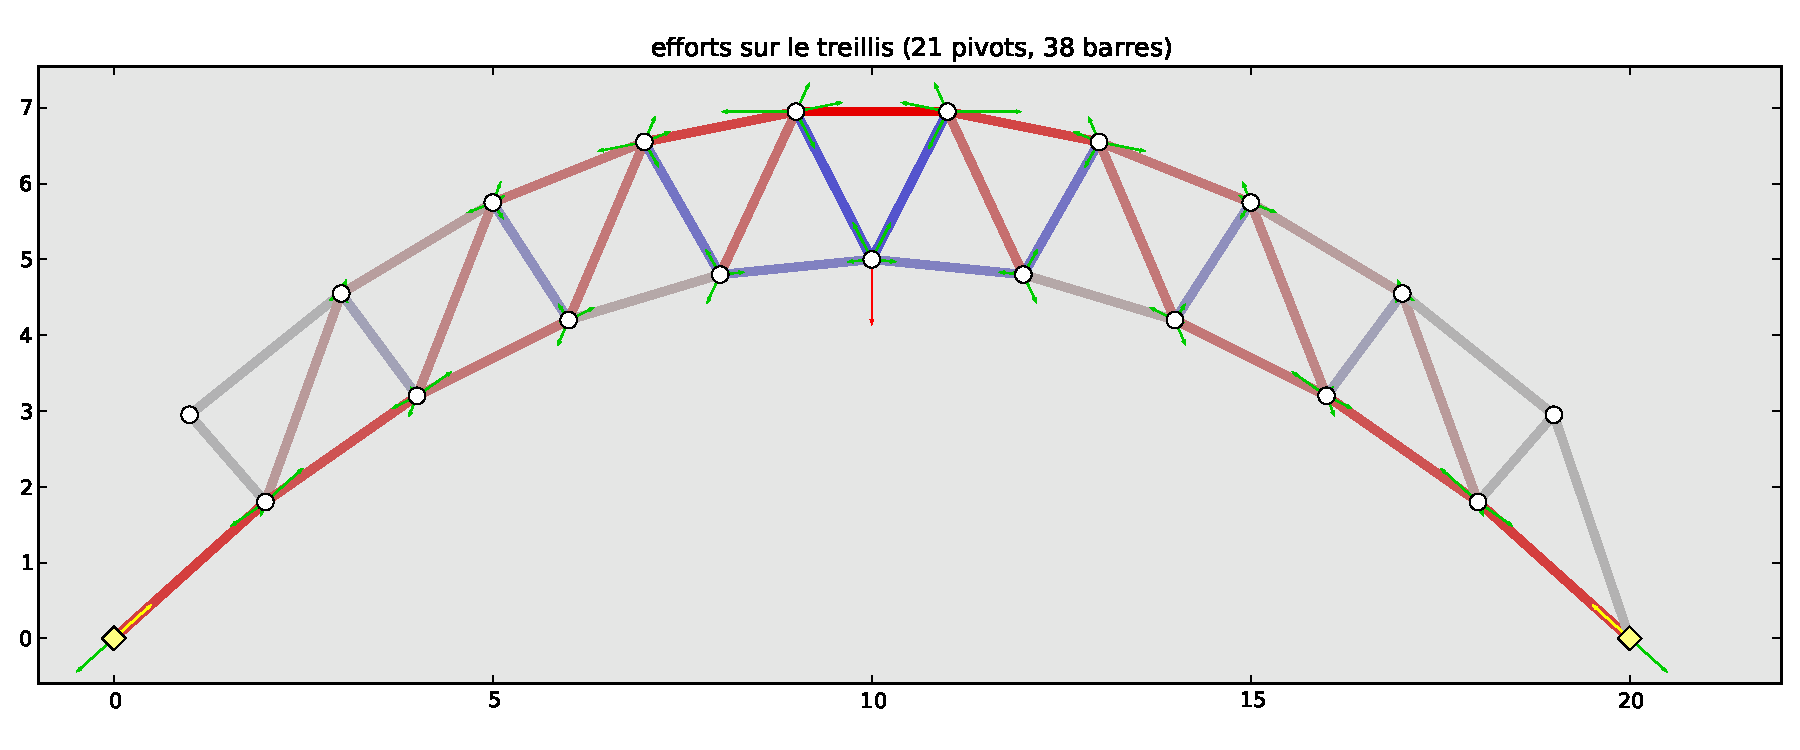
\includegraphics[width=1\textwidth]{treillis_21piv_parabole2.pdf}
    \end{center}
     
  \end{frame}
  
  \begin{frame}
    \frametitle{Le langage Python}
    
    Historique en 2 lignes :
    
    \begin{itemize}
     \item Création de Python : années 1990 (Guido van Rossum)
     \item Écosystème Python numérique : années 2000
    \end{itemize}
    
    \vspace{1em}
    
    Python est un langage de programmation \emph{open source}, \emph{dynamique} et \emph{généraliste}.
    Il est utilisé pour réaliser des sites web (YouTube), des interfaces graphiques,
    l'automatisation de tests dans l'industrie, \dots
    
    \vspace{1em}
    
    \dots{ } et grâce au travail d'une communauté active
    qui a développé des extensions (NumPy, Matplotlib, \dots),
    Python est très utilsé pour
    le \emph{calcul scientifique} (CERN, astronomie, neuro-biologie, \dots)
    
  \end{frame}

  
  \begin{frame}
    \frametitle{Le langage Python}
    \framesubtitle{Pourquoi j'utilise ce langage dans mon travail de thèse}
    
    $\heartsuit$ Un langage dynamique avec une syntaxe claire mais solide.
    
    \vspace{1em}
    
    $\heartsuit$ Un même langage pour faire du calcul numérique et du non-numérique
    (interfaces graphiques, bases de données, \dots).
    
    \vspace{1em}
    
    $\heartsuit$ Une communauté open source dynamique qui crée et fait évoluer des outils
    numériques à la pointe (calcul et visualisation)
    
    \vspace{1em}
    
    \begin{center}
     
\includegraphics[width=0.5\textwidth]{python-logo.png}
    
     \textcolor{gray}{(plus de pub sur \url{http://brochure.getpython.info/} )}
    \end{center}

  \end{frame}
  
  \begin{frame}
    \frametitle{Le langage Python}
    
    \centering \Large
    
    \textcolor{blue}{ \emph{Il est l'heure de commencer !} }
    
    \vspace{2em}
    
    
\includegraphics[width=0.5\textwidth]{python-logo.png}

    
  \end{frame}
  

\end{document}
